\documentclass[12pt,hyperref={CJKbookmarks=true}]{beamer}
\usepackage[adobefonts,noindent,space]{ctex}
\usepackage{amsmath}
\usepackage[timeinterval=1]{tdclock} %使用数字时钟宏包
\graphicspath{{mask/}{process/}{unrecognised/}}
\usetheme{Warsaw}
\begin{document}
\title{电流表读数自动识别}
\author[何为]{何为(0943041105)\\[10pt] \small指导教师:张蕾}
\institute{计算机学院}
\date{2013年5月26日}
\logo{\tiny\LaTeX}

\begin{frame}
  \titlepage
\end{frame}

\section{绪论}

\begin{frame}
  \frametitle{选题原因}
  \begin{columns}[onlytextwidth]
    \begin{column}{0.6\textwidth}
      \begin{itemize}
      \item 数量多,位置分散
      \item 处于高压环境中
      \item 需要实时监控
      \item 难以换成电子式电流表
      \end{itemize}
    \end{column}
    \begin{column}{0.4\textwidth}
      \centering
      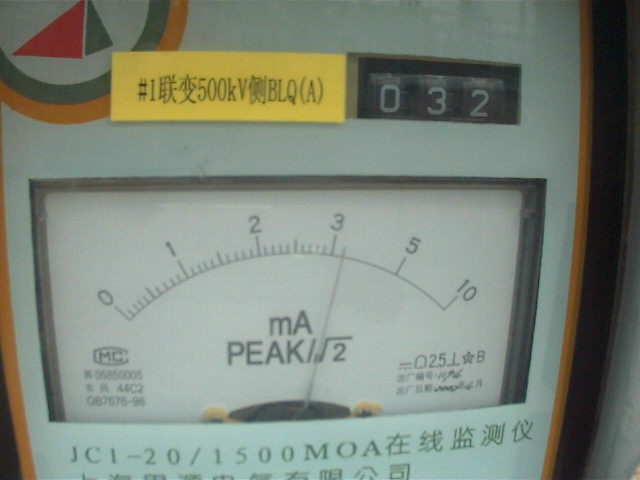
\includegraphics[width=0.9\textwidth]{src.png}
    \end{column}
  \end{columns}
\end{frame}

\begin{frame}
  \frametitle{电流表图像特点}
  \begin{columns}[onlytextwidth]
    \begin{column}{0.6\textwidth}
      \begin{itemize}
      \item 数字形状和大小一致
      \item 数字只占很小的一部分
      \item 数字在黑色边框中
      \item 防护玻璃反光
      \item 数字边框的背景亮度不均匀
      \end{itemize}
    \end{column}
    \begin{column}{0.4\textwidth}
      \centering
      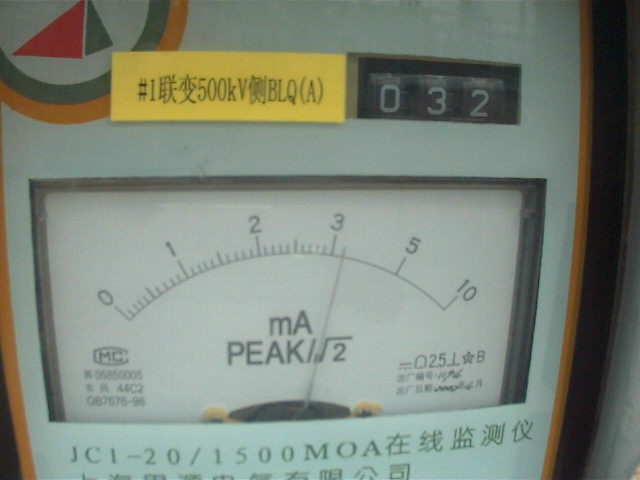
\includegraphics[width=0.9\textwidth]{src.png}
    \end{column}
  \end{columns}
\end{frame}

\begin{frame}
  \frametitle{识别过程}
  \begin{enumerate}
  \item \textbf{预处理}:减少噪声和干扰
  \item \textbf{数字边框定位}:找出数字的大致位置
  \item \textbf{数字分割}:分割成单个的数字
  \item \textbf{数字识别}:识别每个数字
  \end{enumerate}
\end{frame}
\section{图像预处理}


\begin{frame}
  \frametitle{灰度化}  
  \begin{center}
    取右上部分,$I=0.114R+0.587G+0.299B$
  \end{center}
  \begin{columns}[onlytextwidth]
    \begin{column}{0.5\textwidth}
      \centering
      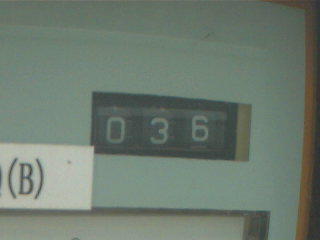
\includegraphics[width=0.9\textwidth]{rgb.png}\\
      \footnotesize 彩色图像
    \end{column}
    \begin{column}{0.5\textwidth}
      \centering
      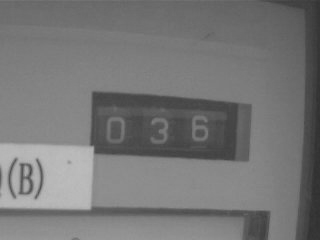
\includegraphics[width=0.9\textwidth]{gray.png}\\
      \footnotesize 灰度图像
    \end{column}
  \end{columns}
\end{frame}

\begin{frame}
  \frametitle{高斯滤波}
  \begin{columns}[onlytextwidth]
    \begin{column}{0.5\textwidth}
      \centering
      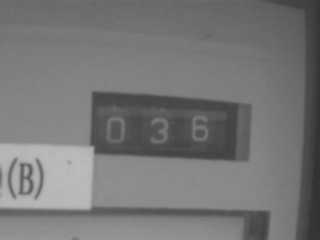
\includegraphics{gaussian.eps}\\
      \footnotesize 模板
    \end{column}
    \begin{column}{0.5\textwidth}
      \centering
      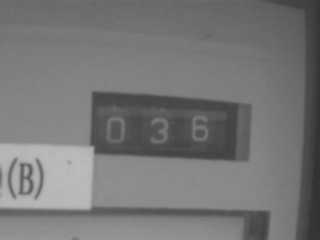
\includegraphics[width=0.9\textwidth]{gaussian.png}\\
      \footnotesize 效果
    \end{column}
  \end{columns}
\end{frame}

\begin{frame}
  \frametitle{直方图均衡}
  \begin{columns}[onlytextwidth]
    \begin{column}{0.5\textwidth}
      \centering
      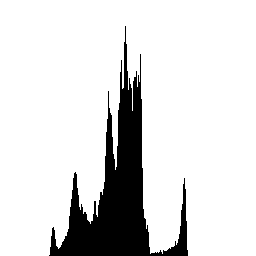
\includegraphics[width=0.9\textwidth]{histsrc.png}\\
      \footnotesize 均衡化前
    \end{column}
    \begin{column}{0.5\textwidth}
      \centering
      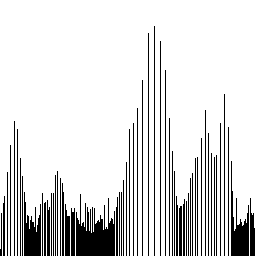
\includegraphics[width=0.9\textwidth]{histequal.png}\\
      \footnotesize 均衡化后
    \end{column}
  \end{columns}
\end{frame}

\section{数字边框定位}

\subsection{二值化}


\begin{frame}
  \frametitle{二值化}
  \begin{block}{算法}
    Otsu算法
  \end{block}
  \begin{block}{原理}
    使类间方差$\sigma_B^2(t)=q_1(t)q_2(t)[\mu_1(t)-\mu_2(t)]^2$最小
  \end{block}
  \begin{block}{计算方法}
    在$t$的\textbf{有效范围}内用递推公式计算$q_1(t),q_2(t),\mu_1(t),\mu_2(t)$四项
  \end{block}
\end{frame}

\begin{frame}
  \frametitle{Otsu算法效果}
  \begin{columns}[onlytextwidth]
    \begin{column}{0.5\textwidth}
      \centering
      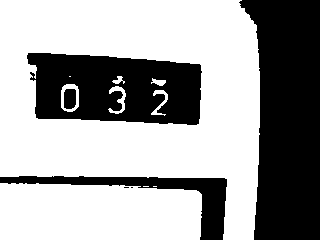
\includegraphics[width=0.9\textwidth]{otsu.png}
    \end{column}
    \begin{column}{0.5\textwidth}
      \begin{itemize}
      \item 黑色区域和白色区域
      \item 边框轮廓准确
      \item 数字分割不准确
      \end{itemize}
    \end{column}
  \end{columns}
\end{frame}

\subsection{连通成分筛选}

\begin{frame}
  \frametitle{连通成分标记}
  \begin{columns}[onlytextwidth]
    \begin{column}{0.5\textwidth}
      两轮扫描
      \begin{enumerate}
      \item 赋予临时标记
      \item 替换成等价标记
      \end{enumerate}      
    \end{column}
    \begin{column}{0.5\textwidth}
      \centering
      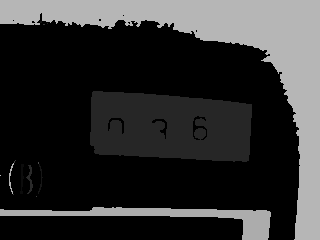
\includegraphics[width=0.9\textwidth]{candidate.png}
    \end{column}
  \end{columns}
\end{frame}

\begin{frame}
  \frametitle{连通成分筛选}
  \begin{columns}[onlytextwidth]
    \begin{column}{0.5\textwidth}
      特征:
      \begin{itemize}
      \item 像素数$n$
      \item 长宽比$r=L/w$
      \item 密度$\rho=n/S$
      \end{itemize}
    \end{column}
    \begin{column}{0.5\textwidth}
      范围:
      \begin{equation*}
        \begin{aligned}
          8000 < &n < 10000 \\
          1.9 < &r < 2.9 \\
          0.6 < &\rho < 0.9
        \end{aligned}
      \end{equation*}
    \end{column}
  \end{columns}
\end{frame}

\subsection{倾斜校正}

\begin{frame}
  \frametitle{倾斜校正}
  \begin{columns}
    \begin{column}{0.3\textwidth}
      \centering
      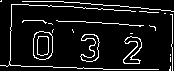
\includegraphics[width=0.9\textwidth]{canny.png}\\
      \footnotesize Canny边缘检测算子
    \end{column}
    \begin{column}{0.3\textwidth}
      \centering
      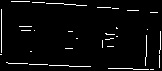
\includegraphics[width=0.9\textwidth]{hough.png}\\
      \footnotesize 哈夫变换
    \end{column}
    \begin{column}{0.3\textwidth}
      \centering
      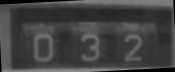
\includegraphics[width=0.9\textwidth]{rotate.png}\\
      \footnotesize 旋转图像
    \end{column}
  \end{columns}
\end{frame}

\section{数字分割}

\subsection{二值化}

\begin{frame}
  \frametitle{动态阈值法}
  \begin{block}{原因}
    背景灰度不均匀
  \end{block}
  \begin{block}{原理}
    在每个邻域内分别计算阈值
  \end{block}
  \begin{block}{阈值计算方法}
    高斯滤波均值加上常数$C=1.5$
  \end{block}
\end{frame}

\subsection{形态学运算}


\begin{frame}
  \frametitle{形态学运算}
  \begin{center}
    原因:二值化图像含有噪声,部分数字内部有空隙
  \end{center}
  \begin{columns}[onlytextwidth]
    \begin{column}{0.5\textwidth}
      \centering\includegraphics[width=0.5\textwidth]{cross.eps}\\
      \footnotesize 形态学结构元
    \end{column}
    \begin{column}{0.5\textwidth}
      \centering
      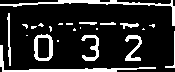
\includegraphics[width=0.5\textwidth]{framebin.png}\\
      \footnotesize 结果
    \end{column}
  \end{columns}
\end{frame}

\subsection{数字定位}

\begin{frame}
  \frametitle{投影法}
  \begin{columns}[onlytextwidth]
    \begin{column}{0.5\textwidth}
      \begin{enumerate}
      \item \textbf{消除背景噪声}:对各处投影的像素数进行排序,找出中间处的像素数,减去该处像素数。
      \item \textbf{寻找波峰}:用高阈值找出尖峰,用低阈值找出尖峰两侧的部分。
      \end{enumerate}
    \end{column}
    \begin{column}{0.5\textwidth}
      \centering
      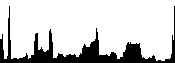
\includegraphics[width=0.5\textwidth]{projectx.png}\\
      \footnotesize 含噪声的投影\\
      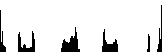
\includegraphics[width=0.5\textwidth]{proclear.png}\\
      \footnotesize 消除噪声的投影\\[5pt]
      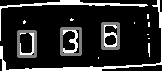
\includegraphics[width=0.5\textwidth]{segment.png}\\
      \footnotesize 数字定位
    \end{column}
  \end{columns}
\end{frame}

\section{数字识别}

\subsection{归一化}


\begin{frame}
  \frametitle{步骤}
  \begin{enumerate}
  \item \textbf{位置归一化}:计算数字的质心,将图像的中心平移至质心。
  \item \textbf{大小归一化}:将数字的长宽缩放至模板的大小。
  \item \textbf{笔画粗细归一化}:用Hilditch算法细化笔画至一像素宽。
  \end{enumerate}
\end{frame}

\subsection{模板匹配}


\begin{frame}
  \frametitle{模板制作}
  \begin{block}{方法}
    从分割的数字中,找出大小和形状最理想的,归一化成$16\times 27$大小
  \end{block}
  \begin{block}{问题}
    数字“1”太窄,归一化后横向拉伸形变严重,不宜作为模板
  \end{block}
  \begin{block}{解决方法}
    判断是否为细长的直线判断是否为“1”
  \end{block}
\end{frame}

\begin{frame}
  \frametitle{匹配方法}
  \begin{block}{原理}
    用Hausdorff距离衡量待识别字符和模板的差距
  \end{block}
  \begin{block}{定义}
    \begin{equation*}
      \begin{aligned}
        h(A,B)&=\max_{a\in A}\min_{b\in B}||a-b||\\
        h(B,A)&=\max_{b\in B}\min_{a\in A}||a-b||\\
        H(A,B)&=\max(h(A,B),h(B,A))
      \end{aligned}
    \end{equation*}
  \end{block}
\end{frame}

\section{效果}

\begin{frame}
\frametitle{识别率}
  在47张电流表图像中
  \begin{itemize}
  \item 40张正确识别,识别率为85.1\%
  \item 未正确识别的7张中
    \begin{itemize}
    \item 4张数字边框定位不准确
    \item 2张数字分割错误
    \item 1张将竖直干扰线误认为数字“1”
    \end{itemize}
  \end{itemize}
\end{frame}
\begin{frame}
  \frametitle{未正确识别的图像}
  \begin{columns}[onlytextwidth]
    \begin{column}{0.3\textwidth}
      \centering
      \includegraphics[width=\textwidth]{unrec1.png}\\
      \footnotesize 阳光强烈
    \end{column}
    \begin{column}{0.3\textwidth}
      \centering
      \includegraphics[width=\textwidth]{unrec2.png}\\
      \footnotesize 未对焦
    \end{column}
    \begin{column}{0.3\textwidth}
      \centering
      \includegraphics[width=\textwidth]{unrec3.png}\\
      \footnotesize 反光严重
    \end{column}
  \end{columns}
\end{frame}
\end{document}
%%% Local Variables: 
%%% mode: latex
%%% TeX-master: t
%%% End: 
